\chapter{Material e Métodos}

\section{Material}

O ferro fundido nodular utilizado neste trabalho foi fundido pela empresa Tupy S/A. O material foi fundido na forma de blocos em Y conforme especificação da norma NBR 6916 (Figura \ref{fig:nbr6916}) para extração de corpos de prova para ensaios mecânicos. A liga foi fundida em forno de indução a cadinho com capacidade de nove toneladas e operado em frequência de rede. Os blocos foram vazados em moldes confeccionados em processo de caixa fria (areia de sílica com resina fenólica uretânica).

\begin{figure}
  \includegraphics[width=12cm]{img/nbr6916.pdf}
  \caption{Desenho esquemático do bloco em Y especificado pela norma NBR 6916 para extração de corpos de prova de ensaios mecânicos. Dimensões em milímetros.}
  \label{fig:nbr6916}
\end{figure}

Durante o projeto da liga procurou-se utilizar baixos teores de manganês e o maior grau de inoculação possível. Estas medidas foram tomadas de forma a minimizar a microsegregação inerente ao processo de fundição. Adicionalmente, o metal líquido foi submetido a processo de inoculação durante o vazamento e \enfase{em molde}, o que permitiu a obtenção de uma liga com elevada contagem de nódulos de grafita, superior a 400 nódulos/mm\textsuperscript{2}. A composição química da liga é dada na Tabela \ref{tab:CQ}. %será que eu falo a contagem de nódulos obtida aqui ou na parte de resultados?

\begin{table}
  \caption{Composição química da liga fundida (\% em massa).}
  \begin{tabular}{c c c c c c c c c}
  \thickhline
  \textbf{Elemento} & C & Si & Mn & Cu & Cr & Mg & P & S \\
  \hline
  \textbf{Composição (\% em massa)} & 3,47 & 2,47 & 0,20 & 0,38 & 0,03 & 0,03 & 0,04 & 0,01 \\
  \thickhline
  \end{tabular}
  \label{tab:CQ}
\end{table}

\section{Metodologia}

\subsection{Determinação dos parâmetros de tratamentos térmicos}

Este estudo se limitou a avaliar o efeito das variáveis ``temperatura de têmpera'' e ``temperatura de partição'' na microestrutura do produto final, na cinética de redistribuição de carbono durante a etapa de partição e na retenção de austenita retida após o processo T\&P. Nesta avaliação, as demais variáveis de tratamento térmico, como a ``temperatura de austenitização'', foram mantidas fixas.

\subsubsection*{Temperatura de austenitização $(T_A)$}

A determinação da temperatura de austenitização do material foi feita utilizando abordagem teórica e experimental. Simulações feitas no software de termodinâmica computacional Thermo-Calc\textregistered{} foram utilizadas para estimar a faixa de temperaturas em que é estabelecido o equilíbrio entre austenita e grafita, na qual é dada a austenitização plena do material. A escolha de uma temperatura muito elevada poderia levar à liquação de regiões do material durante o tratamento térmico. Por outro lado, a escolha de uma temperatura muito baixa poderia levar à austenitização incompleta do material, introduzindo uma variável experimental indesejada.

Para determinação das temperaturas críticas de transformação do material uma amostra de ferro fundido foi submetida a um ensaio de dilatometria no dilatômetro Bähr 805A. A amostra foi aquecida até a temperatura de \SI{880}{\degreeCelsius} a uma taxa de aquecimento de \SI{10}{\degreeCelsius/min} (\SI{0.167}{\degreeCelsius/s}), na qual foi mantida por 5 min antes do resfriamento final a uma taxa de \SI{50}{\degreeCelsius/s}. Mais detalhes sobre as configurações do ensaio de dilatometria são apresentados na seção \ref{subsec:dilatometria}. Os resultados deste experimento preliminar foram comparados com os resultados da abordagem feita pelo software Thermo-Calc\textregistered{}.

O tempo de austenitização escolhido foi de 30 minutos. Embora alguns trabalhos na literatura utilizem tempos mais prolongados para a austenitização plena de ferros fundidos \cite{Trudel1997}, assume-se que, devido ao alto grau de inoculação da liga estudada (cerca de quatro vezes maior do que o utilizado em ligas comerciais), o tempo empregado neste trabalho pode ser considerado suficiente para dissolução das fases presentes na matriz do material na condição como recebida.

\subsubsection*{Temperaturas de têmpera $(T_T)$} 

Como objeto de estudo, foram escolhidas três diferentes temperaturas de têmpera para realização dos tratamentos térmicos: 140, 170 e \SI{200}{\degreeCelsius}. Procurou-se garantir que as três temperaturas utilizadas fossem menores que a temperatura Ms (\SI{230}{\degreeCelsius}), de modo que quantidades substanciais de martensita atérmica fossem produzidas durante a etapa de têmpera. Por sua vez, a determinação da temperatura Ms foi feita preliminarmente por meio de um ensaio de dilatometria que reproduziu o ciclo de austenitização e têmpera.

\subsubsection*{Temperaturas de partição $(T_P)$}

Três diferentes temperaturas de partição foram utilizadas neste estudo: 300, 375 e \SI{450}{\degreeCelsius}. Estas temperaturas foram escolhidas por serem comumente reportadas como parâmetros para os tratamentos isotérmicos na produção do ferro fundido nodular austemperado e por também serem próximas às temperaturas de partição empregadas em aços temperados e particionados.


\subsection{Experimentos de dilatometria}

\label{subsec:dilatometria}

Ensaios de dilatometria foram realizados para a determinação da temperatura Ms da liga estudada --- como mencionado anteriormente --- e para simular os ciclos térmicos correspondentes aos tratamentos de T\&P. Os resultados de dilatometria forneceram informações para identificação das temperaturas de início e fim das transformações de fases durante as etapas de aquecimento e resfriamento e para determinação da cinética das transformações que ocorrem nas etapas isotérmicas do processo T\&P. Os experimentos foram realizados no dilatômetro de têmpera Bähr DIL805A, localizado nas dependências do Departamento de Engenharia Metalúrgica e de Materiais da EPUSP. No dilatômetro o aquecimento das amostras é feito por indução eletromagnética utilizando uma bobina de cobre refrigerada a água e o controle da temperatura é feito por meio de termopares tipo S (Pt/Pt-Rh) soldados às amostras.

Amostras cilíndricas de 10 mm de comprimento e 4 mm de diâmetro foram utilizadas para simular o processo de têmpera e partição nas condições estudadas. As amostras foram usinadas a partir da região central da parte útil do bloco em Y (vide Figura \ref{fig:eletroerosaoBlocoY}), primeiramente por extração por eletroerosão de varetas de 4 mm de diâmetro e em seguida por corte e faceamento para estabelecimento do comprimento útil de 10 mm.

\begin{figure}
  \includegraphics[height=7cm]{img/eletroerosaoBlocoY.pdf}
  \caption{Fotografia da seção de um bloco em Y do material utilizado mostrando os orifícios para retirada dos corpos de prova de dilatometria.}
  \label{fig:eletroerosaoBlocoY}
\end{figure}

O ciclo térmico empregado nos ensaios de dilatometria consistiu da austenitização das amostras por 30 minutos, seguido de rápido resfriamento até a temperatura de têmpera ($T_T$) e reaquecimento até a temperatura de partição ($T_P$), na qual as amostras foram mantidas por entre 30~s e 120~min. As etapas de aquecimento foram realizadas sob taxa de \SI{10}{\degreeCelsius/s}, enquanto a têmpera foi feita a --\SI{50}{\degreeCelsius/s} utilizando resfriamento forçado por gás hélio. A Figura \ref{fig:expDil} representa esquematicamente o ciclo térmico de Têmpera e Partição utilizado ensaios nestes.

\begin{figure}
  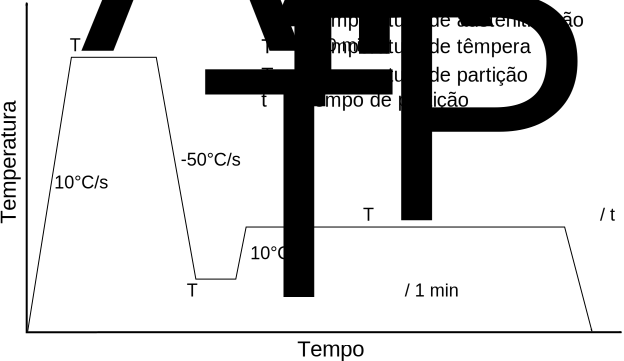
\includegraphics[width=.8\textwidth]{img/expproc_dil.pdf}
  \caption{Ilustração esquemática do ciclo térmico de Têmpera e Partição aplicado nas amostras de dilatometria.}
  \label{fig:expDil}
\end{figure}

O experimento para determinação da temperatura Ms consistiu do aquecimento da amostra até a temperatura de austenitização selecionada, seguindo rampa de aquecimento de \SI{10}{\degreeCelsius/s}, sendo mantida nesta temperatura por 30 minutos. Em seguida, a amostra foi resfriada até a temperatura de \SI{-100}{\degreeCelsius} sob taxa de resfriamento de \SI{50}{\degreeCelsius/s} utilizando gás He refrigerado por $N_2$ líquido. O resfriamento até esta temperatura permitiu que a curva da transformação martensítica fosse determinada por completo. Para que o resfriamento até temperaturas abaixo de zero pudesse ser realizado no equipamento, a geometria da amostra utilizada foi de cilindro perfurado com um furo de diâmetro de \SI{1.5}{mm}.

\subsection{Difração de raios X utilizando radiação síncrotron}

Tratamentos térmicos com acompanhamento em tempo real (\enfase{in situ}) da evolução de fases por difração de raios X (DRX) gerados por fonte de luz síncrotron foram realizados na estação experimental \siglaestrangeira{XTMS}{X-ray Scattering and Thermo-Mechanical Simulation}, operada conjuntamente pelo \sigla{LNNano}{Laboratório Nacional de Nanotecnologia}  e pelo \sigla{LNLS}{Laboratório Nacional de Luz Síncrotron} na cidade de Campinas. A instalação da linha XTMS consiste de um avançado simulador termomecânico integrado à linha de difração de raios X XRD1 no LNLS. O simulador, chamado de Gleeble\textregistered{} 3S50, foi desenvolvido em cooperação da empresa estadunidense \siglaestrangeira{DSI}{Dynamic Systems Inc.} e de corpo técnico-científico do LNNano com o propósito de efetuar testes termomecânicos com controle de temperatura e solicitação mecânica em amostras macroscópicas, enquanto aquisições simultâneas de difração de raios X são obtidas. %A figura xx mostra a configuração da instalação no blablabla

\novasigla{DRX}{Difração de raios X}

No interior da câmara do simulador Gleeble os corpos de prova são presos por garras de cobre, por meio das quais é conduzida corrente elétrica para aquecimento das amostras por efeito Joule. O controle da potência é feito por algoritmo proporcional integral derivativo (PID), sendo que a resposta de temperatura é obtida por meio de termopares (tipo K, Alumel/Cromel) soldados às amostras.

A instalação conta com um goniômetro de alta resolução montado ao redor do simulador. O goniômetro é montado sobre uma mesa de alinhamento que permite o posicionamento do plano de difração sobre a superfície da amostra. Os detetores para contagem de fótons ficam posicionados sobre goniômetro, que pode ser deslocado para ângulos entre 0 e 150° a uma distância mínima de 365 mm da superfície da amostra. Diferentes conjuntos de detectores são disponibilizados na XTMS, permitindo tanto a avaliação em tempo real de frações e parâmetros cristalográficos de fases, como também aquisições com ótimos níveis sinal/ruído. No presente trabalho, detetores 1D Mythen 1K foram utilizados para a análise \enfase{in situ} das transformações de fases durante a etapa de partição, enquanto o detetor 2D Rayonix SX165 foi utilizado para aquisições \enfase{ex situ} (isto é, após os tratamentos térmicos) de amostras tratadas termicamente pelo processo T\&P. Tempos longos de aquisição permitiram a obtenção de difratogramas com excelentes níveis de sinal/ruído, possibilitando a identificação de picos de difração de baixa intensidade, associados a carbonetos.

Dois detetores Mythen 1K, cada um possuindo 1280 canais de aquisição (pixels) de 50 $\mu$m de largura, foram utilizados para as medidas \enfase{in situ}. Na distância mínima de trabalho, cada detetor cobre uma faixa de ângulos de aproximadamente 10°, totalizando um ângulo de cobertura de cerca de 20°. Corpos de prova do ferro fundido foram usinados na geometria esquematizada na Figura \ref{fig:CPXTMS}. Durante o posicionamento das amostras no interior da câmara do simulador procurou-se estabelecer o ângulo $\omega$ de 15° entre a superfície da amostra e o feixe incidente de raios X. Em sequência, as amostras foram submetidas a ciclos de Têmpera e Partição segundo as condições de tratamento térmico pré-determinadas.

Assim como nos ensaios de dilatometria realizados no dilatômetro Bähr, as amostras foram austenitizados durante 30 min, resfriadas até as temperaturas de têmpera e em seguida reaquecidas até as temperaturas de partição, sendo mantidas por 2~h. Nas etapas de resfriamento não foi utilizado resfriamento forçado por meio convectivo, de modo que a extração de calor foi feita unicamente por meio das garras de cobre em contato com os corpos de prova. Consequentemente, taxas de resfriamento inferiores às obtidas no dilatômetro Bähr foram conseguidas no simulador Gleeble. De toda forma, análise metalográfica posterior mostrou que a taxa de resfriamento utilizada foi suficiente para garantir a transformação martensítica na etapa de têmpera.

\begin{figure}
  \includegraphics[width=.9\textwidth]{img/CPXTMS.pdf}
  \caption{Desenho esquemático do corpo de prova utilizado na estação experimental XTMS. Dimensões em  milímetros.}
  \label{fig:CPXTMS}
\end{figure}

As medidas em tempo real de difração de raios X foram realizadas utilizando a energia de feixe de 12 keV, equivalente ao comprimento de onda $\lambda = 1,033\text{\AA}$. O feixe branco gerado pelo anel síncrotron consiste de fótons com uma gama de energias. O feixe monocromático para o experimento de DRX é obtido por meio de um par de cristais monocromadores de Si(111) posicionados no começo da linha de difração. Fendas de limitação de fluxo de fótons foram ajustadas para permitirem que apenas uma região de 2 x 0,5 mm\textsuperscript{2} do feixe incidisse sobre a superfície da amostra. A Figura \ref{fig:esqXRD1} ilustra esquematicamente esse sistema de condicionamento do feixe. Durante as aquisições em tempo real, o goniômetro foi fixado no ângulo 2$\theta$ de 31° e os detetores Mythen foram aproximados até a distância mínima de trabalho de 365 mm. Nesta configuração, os detetores puderam cobrir uma faixa de ângulos de difração entre 26 e 47°, na qual foi possível monitorar a evolução dos picos de difração (110) e (200) da ferrita e (111) e (200) da austenita em tempo real. 
% Embora o material possua grande quantidade de grafita, picos de difração desta fase não foram monitorados, nem visualizados nos difratogramas. Isto ocorre porque como o carbono é um elemento muito leve, sua seção de choque em relação ao fóton é muito baixa. Dessa forma, ainda que hajam picos desta fase, caso o tempo de exposição do detetor não seja suficientemente grande, eles são confundidos com o ruído de fundo do sinal.

\begin{figure}
  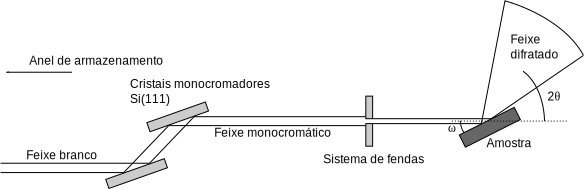
\includegraphics[width=\textwidth]{img/XRD1.pdf}
  \caption{Representação do sistema de condicionamento do feixe de raios X para os experimentos de DRX \textit{in situ} na estação XTMS. Os ângulos $\omega$ da superfícies da amostra com o feixe e o ângulo de Bragg $2\theta$ do feixe difratado são também representados.}
  \label{fig:esqXRD1}
\end{figure}


Dependendo da etapa do tratamento térmico, foram utilizados diferentes tempos e frequências de aquisição de dados. Durante a etapa isotérmica de partição, cuja análise é enfatizada neste trabalho, aquisições foram feitas usando tempo de exposição de 3 segundos, espaçadas a cada 0,5 segundos. Ao final da etapa de partição e do tratamento térmico foram feitas varreduras do ângulo de difração entre 26 e 86° a 10 segundos de exposição por passo, de modo a obter um número de picos de difração substantivo para quantificação das fases. A Figura \ref{fig:esqXTMS} ilustra a programação do experimento na instalação XTMS.

\begin{figure}
  \includegraphics[height=10cm]{img/expproc_XTMS.pdf}
  \caption{Ilustração esquemática do teste programado na instalação XTMS.}
  \label{fig:esqXTMS}
\end{figure}

Antes de cada experimento a câmara do simulador Gleeble foi evacuada por um sistema de vácuo composto de bomba mecânica e difusora. Os níveis de vácuo atingidos foram consistentemente inferiores a $1 \times 10^{-2}$ torr. Um bom nível de vácuo é imprescindível para que a oxidação e a descarbonetação do material em sua superfície sejam evitadas durante o aquecimento e a aquisição dos difratogramas.

O detector Rayonix SX165, utilizado para experimentos \enfase{ex situ}, consiste de um detector 2D de alta resolução, com uma área ativa circular de \SI{165}{mm} de diâmetro e pixels de tamanho $39 \times \SI{39}{\mu m^2}$. A grande vantagem do detector Rayonix em relação ao detector Mythen é a maior quantidade de informação que é possível de ser obtida em uma única aquisição. Como o Rayonix cobre uma área, cada aquisição fornece seções dos anéis de difração, como mostrado na Figura \ref{fig:Rayonix_PT300}a. As maiores desvantagens são os mais longos tempos de aquisição e de leitura. O tempo de leitura pode ser diminuído alterando o \enfase{binning} do detector. O \enfase{binning} permite que pixels ajacentes sejam combinados, diminuindo a resolução do detector, mas também diminuindo o tempo de leitura. Dessa forma, um \enfase{binning} de $2 \times 2$ significa que quatro pixels adjacentes em uma janela $2 \times 2$ no detector são combinados para formar um único pixel na saída de aquisição. As aquisições brutas obtidas consistem de imagens 16 bits, correspondentes a $2^{16} = 65536$ tons de cinza, representando a contagem de fótons em cada pixel. 
As aquisições \enfase{ex situ} foram feitas utilizando \enfase{binning} de $2 \times 2$ e tempo de aquisição de 1~min, permitindo excelentes níveis de sinal/ruído.

\begin{figure}
  \centering
  \subfloat[]{\begin{minipage}[c][.5\textwidth]{0.35\textwidth}%
  \includegraphics[width=\textwidth]{img/XTMS/PT300_detector.pdf}
  \end{minipage}}
  \quad
  \subfloat[]{\begin{minipage}[c][.5\textwidth]{0.6\textwidth}%
  \includegraphics[width=\textwidth]{img/XTMS/PT300_spherical.pdf}
  \end{minipage}}
  \vspace{0pt}
  \subfloat[]{\includegraphics[width=.7\textwidth]{img/XTMS/PT300_diffractogram.pdf}}
  \caption{Sequência de etapas para conversão da imagem obtida pelo detector Rayonix em difratograma. (a) Imagem original. (b) Dados de aquisição representados em coordenadas polares. (c) Difratograma obtido pela integração dos dados ao longo do ângulo azimutal.}
  \label{fig:Rayonix_PT300}
\end{figure}

Uma vez feita a aquisição, a imagem bruta adquirida é processada de modo a converter as coordenadas retangulares do detector para coordenadas esféricas representando os ângulos de difração. Este processo é feito utilizando um \enfase{script} escrito em python que reimplementa o algoritmo originalmente desenvolvido pela equipe da XTMS em Matlab\footnotemark. A Figura \ref{fig:Rayonix_PT300}b representa os dados da aquisição mostrada na Figura \ref{fig:Rayonix_PT300}a no novo sistema de coordenadas esféricas. O eixo das abcissas corresponde ao ângulo azimutal, que pode fornecer informações sobre a orientação cristalográfica do material (e.g., textura), enquanto o eixo das ordenadas representa o ângulo de Bragg $2 \theta$.

\footnotetext{Daniel Candeloro Cunha. Apresentação CPM. LNNano, 28 de Julho de 2015}

O objetivo dos experimentos \enfase{ex situ} é apenas identificar e quantificar as fases presentes, de modo que as informações que o ângulo azimutal fornecem são redundantes. Dessa forma, é mais conveniente que os picos de difração sejam integrados ao longo do ângulo azimutal, tendo como resultado final um difratograma convencional, em que as intensidades são representadas em função do ângulo de Bragg $2\theta$, como mostrado na Figura \ref{fig:Rayonix_PT300}c. Por fim, o sinal de fundo é ajustado e removido para melhor visualização dos picos e quantificação de fases. Essas etapas são também realizada utilizando um \enfase{script} implementado em python.

\subsubsection{Análise dos resultados de DRX}

\label{subsec:analiseDRX}

Uma vez que a amostra fica posicionada em um ângulo $\omega$ fixo em relação ao feixe de raios X, a geometria de difração $\omega$--$2\theta$ utilizada difere fundamentalmente das geometrias convencionais dos métodos de Bragg-Brentano ($\theta$--$2\theta$) e Debye-Scherrer (feixe transmitido). A interpretação dos padrões de difração, no entanto, seguiu procedimentos semelhantes de indexação e determinação dos parâmetros de rede das fases.

A análise dos difratogramas obtidos durante os tratamentos isotérmicos foi feita por meio de rotinas programadas em R. Os picos de difração obtidos foram ajustados segundo a equação de distribuição Gaussiana (equação \ref{eq:Gaussiana}) que representa uma função sino que descreve o formato dos picos de difração. O autor é ciente que para esta tarefa costuma ser utilizada uma função do tipo Pseudo-Voigt, que descreve melhor o alargamento instrumental associado aos picos de difração. Todavia, devido ao custo de processamento computacional e problemas no ajuste de picos superpostos utilizando essa função, optou-se pelo uso de perfis Gaussianos, que demonstraram fornecer resultados satisfatórios.

\begin{equation}
  I = I_0 \exp{\left[-\left(\frac{2\theta - 2\theta_0}{w}\right)^2\right]} + bck
  \label{eq:Gaussiana}
\end{equation}

Na equação \ref{eq:Gaussiana}, $I$ corresponde à intensidade de difração observada em função do ângulo $2\theta$, $I_0$ é a intensidade máxima medida no ângulo de difração $2\theta_0$, $w$ é a largura do pico Gaussiano e $bck$ contabiliza o sinal de fundo (\enfase{background}), que tem seu valor assumido como constante. As áreas integradas ($A_{hkl}$) sob os picos foram calculadas pela integração da curva Gaussiana usando a equação \ref{eq:intGauss}, sendo convertidas para frações volumétricas de fases pela equação \ref{eq:fracDRX}, conforme metodologia descrita por \citaremsentenca{Cullity2001}.

\begin{align}
  A &= \int\limits_{-\infty}^{\infty} I_0 \exp{\left[-\left(\frac{2\theta - 2\theta_0}{w}\right)^2\right]} d \theta \nonumber \\
  &= I_0 |w| \sqrt{\pi}
  \label{eq:intGauss}
\end{align}

\begin{equation}
  f^\gamma = 1 - f^\alpha = \frac{\sum A_{hkl}^\gamma/R_{hkl}^\gamma}{\sum A_{hkl}^\alpha/R_{hkl}^\alpha + \sum A_{hkl}^\gamma/R_{hkl}^\gamma}
  \label{eq:fracDRX}
\end{equation}

A equação \ref{eq:fracDRX} faz uso dos coeficientes $R_{hkl}$, que consistem das intensidades teóricas calculadas para cada fase. A contabilização de $R_{hkl}$ passa pelo produto de vários fatores instrumentais e ambientais que contribuem para a intensidade do feixe espalhado. Comumente é possível expressar $R_{hkl}$ pela contribuição de três principais fatores, estrutura ($F_{hkl}$), Lorentz-Polarização ($LP$) e multiplicidade [de planos] ($p$), como mostra a equação a seguir:

\begin{equation}
  R_{hkl} = \left| F_{hkl} \right|^2 \cdot LP \cdot p
  \label{eq:Rhkl}
\end{equation}

Neste trabalho, $R_{hkl}$ foi obtido a partir do programa \enfase{open source} PowderCell, que simula difratogramas teóricos a partir das informações cristalográficas da fase e dos parâmetros experimentais (o principal é o comprimento de onda da radiação). Na Tabela \ref{tab:fatoresR} são apresentados os valores de $R_{hkl}$ utilizados para quantificação das fases neste trabalho.

\begin{table} %REVISAR ANTES DE IMPRIMIR!
  \caption{Fatores multiplicidade de planos $p$ e coeficientes $R_{hkl}$ para as fases ferrita ($\alpha$) e austenita ($\gamma$).}
  \begin{tabular}{c c c c | c c c c}
  \hline
  Fase & hkl & p & $R_{hkl}$ & Fase & hkl & p & $R_{hkl}$\\
  \hline
  & 110 & 12 & 253,72 & & 111 & 8 & 188,50\\
  & 200 & 6 & 43,94 & & 200 & 6 & 92,95\\
  $\alpha$ & 211 & 24 & 88,41 & $\gamma$ & 220 & 12 & 61,11\\
  & 220 & 12 & 26,56 & & 311 & 24 & 70,11\\
  & 310 & 24 & 35,68 & & 222 & 8 & 20,02\\
  \hline
  \end{tabular}
  \label{tab:fatoresR}
\end{table}

A variação do parâmetro de rede da austenita ao longo do tratamento isotérmico também foi avaliada pelos resultados de DRX. A partir do cálculo do espaçamento interplanar $d_{hkl}$ pela lei de Bragg (equação \ref{eq:Bragg}), o parâmetro de rede da austenita $a^\gamma$ foi determinado pela equação \ref{eq:parametroRede}, que, para sistemas cristalinos cúbicos, estabelece a relação entre o parâmetro de rede da fase e a distância interplanar entre planos de índices de Miller $hkl$.

\begin{equation}
  n\lambda = 2d_{hkl}\,sen(\theta_0)
  \label{eq:Bragg}
\end{equation}

\begin{equation}
  d_{hkl}^\gamma = \frac{a^\gamma}{\sqrt{h^2 + k^2 + l^2}}
  \label{eq:parametroRede}
\end{equation}

A variação do parâmetro de rede foi interpretada pelo enriquecimento em carbono da austenita durante a etapa de partição do tratamento T\&P. Dessa forma, a variação do teor de carbono foi estimada por meio da equação empírica obtida por \citaremsentenca{Dyson1970}, que leva em conta a variação do parâmetro de rede da austenita em função de sua composição química:

\begin{equation}
  a^\gamma = \SI{3.5780}{} + \SI{3.30e-2}{} \%w_C^\gamma + \SI{9.5e-4}{} \%w_{Mn}^\gamma + \SI{1.5e-3}{} \%w_{Cu}^\gamma
  \label{eq:DysonHolmes}
\end{equation}
%
em que $\%w_j^\gamma$ é a porcentagem em massa do elemento $j$ (= C, Mn, Cu) dissolvido na austenita. A equação original também descreve a contribuição de outros elementos no parâmetro de rede da austenita. No entanto, suas representações na equação acima foram poupadas, devido a seus baixos teores na liga estudada. Dyson e Holmes argumentam que o silício, que aparece em quantidade substancial no ferro fundido, apresenta efeito desprezível na distorção do reticulado da austenita e, por esse motivo, sua contribuição não foi incorporada à equação.

Uma vez que as aquisições foram feitas a temperaturas elevadas, para que os valores de $a^\gamma$ obtidos pelos difratogramas pudessem ser interpretados na temperatura ambiente pelo método descrito acima, previamente à aplicação da equação \ref{eq:DysonHolmes}, o efeito da expansão térmica no parâmetro de rede da austenita foi corrigido utilizando a equação desenvolvida por \citaremsentenca{VanBohemen2013b}:

\begin{equation}
  \frac{\Delta L^\gamma}{L_0^\gamma} = B_\gamma T + B_\gamma \Theta_D^\gamma \left[ \exp{\left( -\frac{T}{\Theta_D^\gamma} \right)}\right]
  \label{eq:expTermica}
\end{equation}

A equação \ref{eq:expTermica} descreve a variação de comprimento $\Delta L^\gamma$ de uma amostra completamente austenítica na temperatura absoluta $T$ em relação a seu comprimento $L_0^\gamma$ extrapolado para o estado de referência a 0 K. $B^\gamma$ e $\Theta_D^\gamma$ são constantes de ajuste determinadas pela regressão linear de dados disponíveis na literatura e valem $B^\gamma = 24,8 \times 10^{-6} K^{-1}$ e $\Theta_D^\gamma = 280 K$.

\subsection{Caracterização microestrutural}

Para análise da microestrutura das amostras, estas foram submetidas a preparação metalográfica, que consistiu do embutimento das amostras em baquelite, lixamento em lixa d'água até granulometria 1200 e subsequente polimento em pastas de diamante de 6, 3 e 1 $\mu$m. Por fim, as amostras foram submetidas a ataque metalográfico utilizando o reagente Nital 2\% (etanol + \SI{2}{\%vol.} $HNO_3$).

As observações metalográficas foram feitas tanto no \sigla{PMT-USP}{Departamento de Engenharia Metalúrgica e de Materiais da EPUSP}, como no grupo de Projeto Microestrutural de Materiais Metálicos Estruturais durante estágio de pesquisa no Instituto para Pesquisa de Materiais da Universidade de Tohoku em Sendai, Japão. As imagens de \sigla{MO}{Microscopia Óptica} foram obtidas em um microscópio Olympus BX60M (no PMT-USP) e em microscópios Nikkon (em Sendai). Imagens de \sigla{MEV}{Microscopia Eletrônica de Varredura} foram obtidas em microscópios de canhão de emissão de campo (MEV-FEG) FEI Inspect F50 (no PMT-USP) e JEOL JSM-7001F (em Sendai). Análises de \sigla{EBSD}{Difração de Elétrons Retroespalhados} foram feitas no MEV-FEG JEOL JSM-7001F utilizando sistema de EBSD TSL OIM. 

\novasigla{FEG}{Canhão de Emissão de Campo}

\subsubsection{Análises de microssonda eletrônica}

\sigla{EPMA}{Análises de Microssonda Eletrônica} foram realizadas no Laboratório de Microssonda Eletrônica do \sigla{IGc-USP}{Instituto de Geociências da USP} utilizando um equipamento com canhão de emissão de campo JEOL JXA-FE-8530. O EPMA permitiu a realização de análise local de variações de composições químicas por meio da técnica de \sigla{WDS}{Espectroscopia de raios X dispersivo de comprimento de ondas}. Análises foram realizadas sob baixa magnificação ($\approx 100\times$) para determinação da distribuição de Mn, Si e Cu associada à microssegregação de solidificação utilizando tensão de aceleração de \SI{15}{keV} e corrente de feixe de \SI{100}{nA}. Nesses experimentos, os ângulos dos cristais analisadores foram ajustados de modo a permitir a determinação da contagem de fótons máxima dos picos de raios X característicos dos elementos analisados (i.e., Mn, Si e Cu). Para quantificação das composições químicas de cada elemento, foram determinadas equações lineares correlacionando a composição do elemento com a contagem de fótons. Para isso, foram utilizadas para cada elemento duas composições de referência: a composição média determinada por análise química (contagem de fótons média) e a composição nos nódulos de grafita, que para estes elementos é sabido que é igual a zero.

Análises em linha também foram feitas sobre altas magnificações ($\approx 5000 \times$) utilizando parâmetros otimizados para a avaliação da distribuição local de carbono. Subsequentemente, as amostras foram atacadas para identificação da microestrutura. As análises de EPMA nestas condição foram feitas utilizando baixos valores de tensão do filamento (\SI{6}{keV}) e da corrente da sonda (\SI{70}{nA}), de modo a minimizar o volume de excitação \cite{Toji2015}. A quantificação da concentração de carbono foi feita por meio de cinco espécimes padrão com teores de carbono variando de 0,2 a 1,2\% em massa. O teor de carbono real de cada amostra foi determinado por análise química pelo método de combustão pelo Laboratório Químico Metais da empresa Falcão Bauer. Para isso, foram extraídos cerca de \SI{10}{g} de cavacos de cada amostra utilizando uma furadeira de mesa. Procurou-se executar este procedimento da forma mais cuidadosa possível --- baixa velocidade de rotação e sem lubrificação --- para evitar a contaminação do material a ser analisado. Na Tabela \ref{tab:comp_padrao_EPMA} são mostradas a origem e o teor de carbono medido em cada amostra. Antes de as amostras padrão serem levadas ao equipamento de EPMA, elas foram tratadas termicamente por austenitização em atmosfera controlada (encapsuladas a vácuo) no campo de austenitização plena (a temperatura de austenitização foi variada de acordo com a composição da liga) e em seguida temperadas até a temperatura ambiente. Este procedimento garante que o carbono no material esteja homogeneizado na forma de martensita supersaturada em carbono. Além disso, as amostras foram seccionadas, embutidas em resina e polidas segundo procedimento metalográfico convencional, de modo a se obter uma superfície plana para análise de EPMA. No equipamento de microssonda, para cada amostra padrão a contagem de fótons relativa ao pico de carbono difratado pelo cristal analisador foi medida usando tensão do filamento de \SI{6}{keV} e corrente da sonda de \SI{70}{nA}.

\begin{table}
  \caption{Informações sobre amostras padrão utilizadas para o levantamento da curva de calibração mostrada na Figura \ref{fig:padrao_EPMA} e expressa pela equação \ref{eq:EPMA_calibracao}. Valores entre parênteses representam o desvio padrão da medida.}
  \begin{tabular}{c c c}
    \thickhline
    \textbf{Liga} & \textbf{Teor de carbono medido} & \textbf{Contagem de fótons (contagens/nA)} \\
    \hline
    SAE 15B26 & 0.261 & 7.76 (0.43) \\
    SAE 1040 & 0.470 & 10.81 (0.71) \\
    SAE 1060 & 0.616 & 11.29 (0.41) \\
    SAE 1080 & 0.703 & 13.69 (0.52) \\
    DIN 125Cr1 & 1.267 & 16.73 (0.59) \\
    \thickhline
  \end{tabular}
  \label{tab:comp_padrao_EPMA}
\end{table}

A Figura \ref{fig:padrao_EPMA} mostra a curva relacionando a contagem de fótons em cada análise e o teor de carbono para a liga correspondente. Este dados foram ajustados por uma equação linear, fornecendo a equação relacionando o teor de carbono local $\%w_C$ com a contagem de fótons medida e a corrente do feixe utilizada:

\begin{equation}
  \%w_C = \SI{-0.6449}{} + \SI{0.1085}{} \frac{contagens}{\text{corrente (nA)}} \label{eq:EPMA_calibracao}
\end{equation}

\begin{figure}
  \centering
  \includegraphics[width=.9\textwidth]{img/EPMA/calibracao_EPMA.pdf}
  \caption{Curva de calibração para medida da composição de carbono por EPMA.}
  \label{fig:padrao_EPMA}
\end{figure}

A equação \ref{eq:EPMA_calibracao} foi aplicada para os conjuntos de dados de análise em linha obtidos nas amostras temperadas e particionadas, fornecendo perfis de composição de carbono.

\simbolo{$T_A$}{Temperatura de austenitização}
\simbolo{$T_T$}{Temperatura de têmpera}
\simbolo{$T_P$}{Temperatura de partição}

\simbolo{$\omega$}{Ângulo entre o feixe de raios X incidente e a superfície da amostra}
\simbolo{2$\theta$}{Ângulo de Bragg} %definir tth melhor aqui.